\documentclass[conference]{IEEEtran}
\usepackage[T1]{fontenc}
\usepackage[utf8]{inputenc}
\usepackage{amsmath,amssymb,amsthm,booktabs,graphicx,microtype}
\usepackage{dblfloatfix}
\usepackage[hidelinks]{hyperref}
\graphicspath{{figures-v2/}}
\newtheorem{proposition}{Proposition}
\newcommand{\R}{\mathbf R}
\newcommand{\E}{\mathbb E}
\title{Spatial and Temporal Entropy for IoT Fault Detection:\\A Comparative Study with Generative References}
\author{\IEEEauthorblockN{Alexander V. Mantzaris and James H. Korris}}
\hypersetup{pdftitle={Spatial and Temporal Entropy for IoT Fault Detection: A Comparative Study with Generative References},pdfauthor={Alexander V. Mantzaris and James H. Korris}}
\begin{document}
\maketitle
\begin{abstract}
% BEGIN GENERATED: abstract
Spatial covariance and within-sensor temporal order describe different aspects
of IoT behavior. We compare local correlation-spectrum, permutation and sample
entropy with conventional spatial and temporal statistics under joint block-bootstrap
and graph-conditioned diffusion references. A frozen extension evaluates
360 fault realizations on 20 simulation/recording blocks with three model seeds,
using one synthetic benchmark and two semi-synthetic real-data benchmarks.
Aligned diagnostics verify that time reordering can preserve covariance while
changing temporal entropy; autocorrelation also detects this distinction.
Results depend on support, reference and calibration. On Intel, bootstrap temporal
entropy achieves recall 0.389 versus 0.000 for the conventional temporal
scan, with respective background exceedance 0.103 and 0.000.
Adding entropy to the conventional combined scan increases synthetic bootstrap
recall by 0.003; other dataset/reference combinations show no recall increase.
Shared-support fidelity exposes substantial diffusion entropy miscoverage.
No consistent overall advantage is established for either entropy or the
generative reference. These exploratory results distinguish feature information
from estimator availability and decision performance, without claiming equivalence.
% END GENERATED: abstract
\end{abstract}
\begin{IEEEkeywords}
IoT, spatial entropy, permutation entropy, sample entropy, diffusion forecasting, fault localization
\end{IEEEkeywords}

\section{Introduction}
Sensor-fed digital twins and data spaces need evidence about changes in both
collective organization and individual dynamics. Copying streams can reduce
independent spatial variation; replay can alter temporal organization without
creating a large marginal outlier. A legitimate operating transition can also
change both. An alert should therefore expose measurements and their provenance,
rather than assert an unverified physical cause.

This study compares information captured by spatial and temporal entropy with
conventional measurements, separating the feature from its normal-reference
model. The motivating connection to Mantzaris's work is specific: entropy
trajectories describe evolving segregation under different network
topologies~\cite{mantzaris2024} and collective flocking
organization~\cite{mantzaris2025}. We transfer attention to evolving organization
and interaction structure. The segregation study uses degree/homophily
distributions; the flocking work develops a thermodynamic description of its
simulation. Here spatial entropy uses normalized correlation eigenvalues,
permutation entropy uses ordinal patterns, and sample entropy uses matching
templates. These definitions differ. We infer neither thermodynamic quantities
nor a second law for sensor recordings.

The earlier version of this project evaluated spatial correlation-spectrum
entropy and established no consistent improvement over its synchronization
comparators. That finding motivates, but does not predetermine, this extension.
A changing spatial-entropy trace is not itself a within-sensor temporal-entropy
estimator. Nor does an unsuccessful reference model establish a limitation of
all entropy features. The original artifacts remain identifiable; new
comparisons, support corrections and diagnostics have separate manifests.

We address six questions. \textbf{RQ1}: does spatial entropy improve detection
or localization over non-entropic spatial statistics? \textbf{RQ2}: do temporal
entropies reveal changes missed by spatial covariance summaries?
\textbf{RQ3}: do they improve over conventional temporal statistics?
\textbf{RQ4}: does combining spatial and temporal evidence improve detection
or localization? \textbf{RQ5}: does a generative reference improve over joint
block bootstrap? \textbf{RQ6}: how do support, missingness, window length,
calibration and mechanism affect these answers?

Our contribution is a reproducible comparison, elementary theoretical
characterization of the information retained by its measurements, and an
inspectable monitoring artifact. We introduce neither an entropy definition
nor a general-purpose diffusion architecture. Conventional features augmented
with entropy are compared directly with conventional features alone; entropy
is not required to win or lose.

\begin{figure}[t]
\centering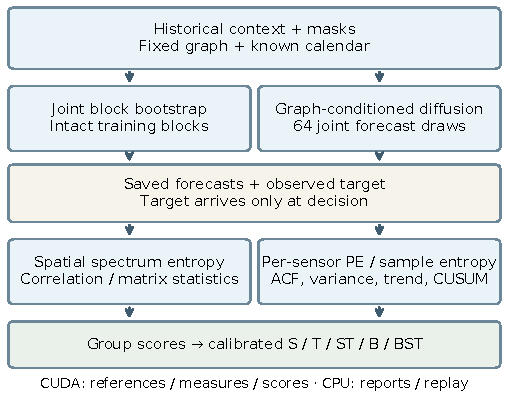
\includegraphics[width=\columnwidth]{architecture.pdf}
\caption{Feature family and normal reference are separate experimental factors.
Both generators issue a joint trajectory before the target; support is applied
after generation. Calibration includes the complete frozen scan family.}
\label{fig:architecture}
\end{figure}

\section{Related Work}
Effective rank measures spectral dimensionality through entropy of normalized
singular values~\cite{effective_rank}; these equal eigenvalues for a PSD
correlation matrix. Graph-entropy anomaly monitoring also predates this
study~\cite{finger}, although a graph Laplacian spectrum differs from the
correlation spectrum used here. Spatial meaning comes from physical/proximity
groups, not from the ordering of sensor columns.

Bandt and Pompe's permutation entropy summarizes neighboring ordinal
patterns~\cite{bandt2002}. Richman and Moorman's sample entropy describes
template-extension regularity~\cite{richman2000}. Their probability objects,
support requirements and amplitude sensitivity differ. Costa et al.'s
multiscale sample entropy~\cite{costa2002} explicitly warns against identifying
irregularity with healthy complexity. We separately label coarse-grained
permutation and sample entropy and make no physiological-health inference.

TimeGrad~\cite{timegrad}, CSDI~\cite{csdi} and DiffSTG~\cite{diffstg} establish
diffusion forecasting, conditional imputation and graph-conditioned generation.
DiffAD~\cite{diffad}, ImDiffusion~\cite{imdiffusion} and
ICDiffAD~\cite{icdiffad} already apply diffusion to anomaly detection. Our
generator uses a forecasting boundary: it receives no measured target value.
GDN~\cite{gdn} supplies a graph-prediction comparator, with adaptation and
information access disclosed below. Dependent-data conformal
work~\cite{conformal} motivates explicit calibration assumptions; we do not
claim a new distribution-free guarantee for an indefinite sensor stream.

\section{Measurements, References and Decisions}
\subsection{Groups, channels and spatial measurements}
Fixed graph-hop neighborhoods have sizes $m\in\{6,12,24\}$ around 24 index-spaced
centers, deduplicated within size. Geographic distance breaks finite hop ties;
node order resolves unreachable nodes when a component is too small. Graphs
represent actual synthetic coupling, Intel coordinate proximity, or release
road distances. Channels remain separate. Main extension windows are
$W\in\{48,96\}$ with $d=W/4$; the original $W=24$ scan is preserved separately.

For one group and channel, retain common complete rows, requiring
$n\geq\max(2m,\lceil.8W\rceil)$. If any column has sample variance at most
$10^{-8}$ in training-scaled units, that group/channel correlation is undefined
and quality-flagged. Otherwise standardize all $m$ columns to sample variance
one, giving $Z$:
\begin{align}
\R_{g,t}&=Z^\top Z/(n-1),\\
\widetilde\R_{g,t}&=(1-\lambda)\R_{g,t}+\lambda I,\\
p_k&=\lambda_k(\widetilde\R_{g,t})/\operatorname{tr}(\widetilde\R_{g,t}),\\[-2mm]
H_S(g,t)&=-\sum_k p_k\log p_k/\log m,\\
\Delta H_S(g,t)&=H_S(g,t)-H_S(g,t-d).
\label{eq:spatial}
\end{align}
Here $0\log0=0$ and $\lambda=.05$. The symmetric eigensolver rejects materially
non-PSD matrices; only roundoff within $64m$ machine epsilons is tolerated.
Gram products disable TF32. This is \emph{local correlation-spectrum entropy},
not entropy of coordinates, thermodynamic states or a degree distribution.

Spatial conventional features are mean signed correlation $C$, mean absolute
correlation, standardized pairwise disagreement $D$, leading concentration
$\lambda_{\max}(\R)/m$, and their lagged changes. With sample-standardized
columns, $D=2(n-1)(1-C)/n$, so it is redundant with $C$ at fixed support.
Full-matrix comparisons include reference-standardized Frobenius discrepancies
of both current $\R$ and $\Delta\R$. A scalar function of $\R$ cannot contain
more information than the full matrix; it may still differ statistically in
estimation or calibration.

\subsection{Per-sensor temporal entropy and support}
We keep each sensor's measurements before group aggregation. For sensor $i$,
use the ordinal vector $v_{i,s}=(x_{i,s+j\tau})_{j=0}^{q-1}$ and estimate its
pattern frequencies $p_{i,t}(\pi)$ in the current window:
\begin{equation}
 H_{\rm PE}(i,t)=-\sum_\pi p_{i,t}(\pi)\log p_{i,t}(\pi)/\log(q!).
 \label{eq:pe}
\end{equation}
The initial configuration is $q=3,\tau=1$; development compares $(3,1),(3,2),(4,1)$.
Missing timestamps invalidate affected templates without compressing time.
Stable temporal-index tie breaking is deterministic. Both endpoints require
at least $\max(30,5q!)$ valid templates; a tied-template fraction above .5 or
a flatline produces an entropy abstention. Tied fractions and a drop-ties
development sensitivity are retained. Ordinal diversity is invariant to a
strict monotone amplitude transformation (up to relabeling patterns); high
entropy does not automatically mean healthy complexity.

For sample entropy, construct complete $(r+1)$-templates with $r=2$. The
common admissible pair set contains unordered starts $a<b$ with $b-a>2$,
excluding self matches and a predeclared Theiler neighborhood. Let $D_r$ be
the maximum distance in the first $r$ coordinates, and $D_{r+1}$ include the
successor. Then
\begin{align}
B_r&=\sum_{(a,b)\in\mathcal P}\mathbf1\{D_r(a,b)\leq\delta\},\\
 A_{r+1}&=\sum_{(a,b)\in\mathcal P}\mathbf1\{D_{r+1}(a,b)\leq\delta\},\\
 H_{\rm SE}(i,t)&=-\log(A_{r+1}/B_r).\label{eq:se}
\end{align}
Both counts use exactly the same valid pairs. Tolerance candidates .1/.2/.3
multiply the sensor's fixed training scale, not its current variance. Development
selects finite-estimate support, with declared tie preferences. We retain
$A,B$, pair and template counts. $B=0$ is undefined; $A=0<B$ is censored/infinite.
Operational scores require 30 templates, $B\geq20$, $A>0$, nonconstant data and
valid endpoints. No pseudocount or arbitrary large finite value replaces an
undefined estimate. This conservative scoring rule can reduce availability;
raw support and censoring remain visible.

For both entropies we compute level and lagged change. Limited multiscale
diagnostics average nonoverlapping bins of sizes 1, 2 and 4 aligned to the left
window boundary. Every bin member must be observed; incomplete final bins are
discarded. The same template criteria apply after coarsening. We do not enlarge
the forecast horizon merely to rescue an unsupported scale. Conventional
comparators receive identical history in these diagnostics.
A separately frozen exploratory sensitivity compares scales 1 and 2 on W96
with the same physical $d=24$, seed-17 episodes and references. It refits scale-2
floors on the original four development issuances and recalibrates each family;
other selected settings are fixed. PE/ACF/Theiler lags use the coarse grid, so
their physical delays double. Spatial measurements retain the original grid.

\subsection{Conventional temporal measurements and feature families}
Temporal baselines include ACF at lags 1, 2 and 4, changes in that ACF vector,
variance of first differences, local sample variance, least-squares trend,
predictive deviation of local mean, and a two-sided within-window CUSUM.
Lag pairs use actual grid positions. Each statistic requires at least
$\max(12,\lceil W/2\rceil)$ points or applicable pairs. CUSUM uses its final state with allowance .5
in training-scaled units, resets at the window start and pauses on missing rows.
Reference scoring below makes these measurements conditional deviations. Raw
predictive residual and the original GDN adaptation remain additional detectors.
Raw residuals average pointwise absolute deviations divided by generated
MAD plus .05, and retain the original spatial-quality restriction. The labeled
GDN adaptation uses 32-dimensional embeddings, learned top-15 neighborhoods,
graph attention and a shared two-layer head, with multiple channels and no
batch normalization. Development-standardized errors average four trailing
one-step predictions, then take a group maximum. It receives causal observed
target history, an information advantage over the long-lead joint references.
Its inherited group support and participation mapping are explicit adaptations,
not a claim to reproduce the authors' published benchmark accuracy.

We report S (spatial entropy), PE and SE separately, T (both temporal
entropies), ST (S plus T), spatial conventional SB, temporal conventional TB,
B (SB plus TB), and BST (B augmented with S and T). Component families combine
by maximum. A family ignores an unsupported component but abstains if none is
available. Each level/change pair itself requires both endpoints. B versus BST
tests incremental benefit rather than only replacement of conventional features.

\subsection{Joint bootstrap and generative references}
Both references generate joint time-by-sensor trajectories, conditioned on a
48-row context ending strictly before the 120-row target. Known calendar
harmonics, coordinates and graph are allowed; future measurements are not.
For a decision at $t$, issuance is $t-120$. The $W=96$ level uses forecast
steps 25--120 and its previous endpoint steps 1--96. The $W=48$ counterparts
use steps 73--120 and 61--108. Thus decision lead is 240 minutes for Intel
and 600 minutes for PEMS, a substantial forecasting challenge. Both feature
endpoints come from the same generated trajectory.

The joint bootstrap chooses intact training blocks using historical-context
and calendar similarity, sampling from the nearest 64 donors. Donor masks
remain. The diffusion model is the original compact DiffSTG/CSDI-inspired
adaptation: width 24, three graph-temporal blocks, historical measurements/masks
and fixed graph/calendar encodings. With Gaussian noise $\epsilon$,
\begin{align}
Y_s&=\sqrt{\bar\alpha_s}Y+\sqrt{1-\bar\alpha_s}\epsilon,\\
\mathcal L_{\rm diff}&=\E\left[
\frac{\|M_{\rm loss}\odot(\epsilon-\epsilon_\theta(Y_s,s,C,G))\|_F^2}
{\sum M_{\rm loss}}\right].\label{eq:diff}
\end{align}
Only valid training targets enter the loss. Original checkpoints use a cosine
schedule~\cite{cosine}, 100 diffusion steps, 20-step DDIM~\cite{ddim}, Adam
$10^{-3}$, batch 8, at most 2400 updates and development early stopping.
Denoised states are clipped to $[-8,8]$ training units; three training seeds
17/29/43 are retained. We do not tune a new architecture on inspected tests.
Each reference supplies 64 draws. Observed masks are imposed after generation,
and additional dropout masks are also applied to the reference measurements.
Bootstrap donor masks can still reduce per-draw rows/templates; common-unit
fidelity comparisons do not claim identical internal estimator support.

\subsection{Scores, group aggregation and calibration}
For feature $a$, set $u_a=(f_a, f_a-f_{a,t-d})$. Componentwise generated medians
$c_{a,t,j}$ and MADs give
\begin{align}
z_{a,t,j}&=\frac{u_{a,t,j}-c_{a,t,j}}
{1.4826\,\operatorname{median}_b|u^{(b)}_{a,t,j}-c_{a,t,j}|+\epsilon_j},\\
A_a(t)&=\max_j|z_{a,t,j}|.\label{eq:score}
\end{align}
Floors for level/change features are $\max(10^{-4},.05\,\mathrm{IQR}_{dev})$.
Legacy matrix-distance and raw-residual comparators retain .01 and .05
regularization floors, respectively. Reference-support counts are retained;
the temporal rule requires at least 52 finite draws, while the retained spatial
summary implementation uses 51 of 64. MAD scaling does not imply Gaussian tails.
Actual $\Delta f$ remains separate from $\Delta f-c_{\Delta f}$.

For each temporal group, average its largest $k=\lceil\eta m\rceil$ valid sensor
scores, requiring at least $\lceil m/2\rceil$ valid members. Fractions
$\eta\in\{.25,.5\}$ and localization budgets in $\{6,12,24\}$ are selected
jointly from four development copy/noise/drift/delay episodes. Mean localization
IoU is pooled over T, TB, ST, B and BST and both references. All families use
the same selected fraction and budget. Max-combined families receive their
own calibration; no uncalibrated union of separately thresholded alerts is used.

With frozen family $\mathcal F$, let $M_t=\max_{a\in\mathcal F}A_a(t)$.
Calibration units are separated by 168 rows (48 context plus 120 target), or
are separate synthetic simulations. For $n_c$ calibration maxima,
\begin{equation}
p_t=\frac{1+\sum_{b=1}^{n_c}\mathbf1\{M_b\geq M_t\}}{n_c+1}.
\label{eq:rank}
\end{equation}
An entirely abstained unit has $M=-\infty$ and cannot alert. Primary
$\alpha=.10$ is fixed before testing. Temporal dependence and distribution
shift can invalidate exchangeability despite gaps; this is a per-issuance
statement, not a stream-wide guarantee. Neither $1-p$ nor a model deviation
is a physical-fault probability. Test controls evaluate background rates;
separate retrospective rate caps are explicitly descriptive, not prospective
threshold validation.

\subsection{Localization and availability}
Group participation weights each group's score by inverse size and normalizes
over eligible incident groups. Direct temporal ranking uses sensor scores;
the combined rule averages their normalized rank percentiles. S/SB use
participation, T/PE/SE/TB direct ranking, and ST/B/BST the combined rule.
All three alternatives are also reported. The budget is selected on development
data, never from test truth. Candidate-group best-overlap IoU is an oracle
diagnostic, not a deployable method. Participation is not causal attribution.

Operational analysis includes every scheduled unit and injected event, including
abstentions and misses. A separately calibrated common-support analysis uses
group/window/channel units valid for S, PE, SE, SB and TB within each reference.
Reference comparisons also report their differing model-support counts; common
feature support is not claimed to eliminate every reference-support difference.
Conditional localization is reported only alongside unconditional scores, where
misses contribute zero. Quality flags, signed agreement and onset alignment
are descriptive and do not create additional uncalibrated detections.

\section{Theoretical and Numerical Characterization}
\begin{proposition}[Bounds and shrinkage]
For a PSD correlation matrix, $0\leq H_S\leq1$. At $\lambda=0$, identity
has entropy one and rank one entropy zero. With positive shrinkage the lower
bound is $-[a\log a+(m-1)b\log b]/\log m$, where
$a=1-\lambda+\lambda/m$ and $b=\lambda/m$.
\end{proposition}
\begin{proof}
The eigenvalues normalized by trace form a probability vector. Shannon
entropy is nonnegative and maximized by uniform probabilities. Shrinkage maps
its simplex into the convex hull of permutations of $(a,b,\ldots,b)$;
concavity makes these extreme points minimizers.\end{proof}

For equicorrelation $\R(\rho)=(1-\rho)I+\rho\mathbf1\mathbf1^\top$,
\begin{equation}
\frac{dH_S}{d\rho}=\frac{m-1}{m\log m}
\log\frac{1-\rho}{1+(m-1)\rho}\leq0,\quad 0\leq\rho<1.
\end{equation}
The eigenvalues are $1+(m-1)\rho$ and $1-\rho$ with multiplicity $m-1$.
Substitution proves the derivative; shrinkage replaces $\rho$ by
$(1-\lambda)\rho$ and multiplies by $1-\lambda$. The displayed nonpositive
sign is restricted to nonnegative $\rho$, not the whole PSD interval.

Entropy need not be determined by average correlation. For $m=4$, compare
equicorrelation .2 with two independent two-sensor blocks of correlation .6.
Both have $C=C_{abs}=.2$ and leading concentration .4, but unshrunk entropies
are .960964 and .860964. Their full matrices distinguish them. This is an
analytic example, not empirical evidence of detector superiority.

\begin{proposition}[Order invariance on an aligned complete window]
For a common time-row permutation $P$, the correlation matrix and its
correlation-spectrum entropy are unchanged.
\end{proposition}
\begin{proof}
Column centering and sample scaling commute with row permutation, and
$(PZ)^\top(PZ)/(n-1)=Z^\top P^\top PZ/(n-1)=Z^\top Z/(n-1)$.
\end{proof}
Order-sensitive temporal measurements can change. This elementary property
applied to measurement design is not a new theorem. It does not imply invariance
of every overlapping rolling window or the whole entropy-change trace. Offsets,
nonzero column gains and sign conjugation also leave the correlation spectrum
unchanged; temporal ordinal entropy can likewise miss amplitude changes.

\begin{proposition}[Conditional rank calibration]
Conditional on a fixed scoring rule, if calibration and next-null maxima are
exchangeable, (\ref{eq:rank}) is super-uniform. Its smallest attainable value
is $1/(n_c+1)$.
\end{proposition}
\begin{proof}
Among $n_c+1$ exchangeable scores the test score's upper rank is uniform in
the absence of ties; including all tied calibration scores makes it
conservative. The trained rule must be fixed before these units.\end{proof}
The premise is not established merely by chronological partitioning. Controlled
null simulations, finite-difference derivatives, explicit CPU pair counts,
CPU/GPU agreement and leakage/event-matching checks accompany the proof.

\begin{figure}[t]
\centering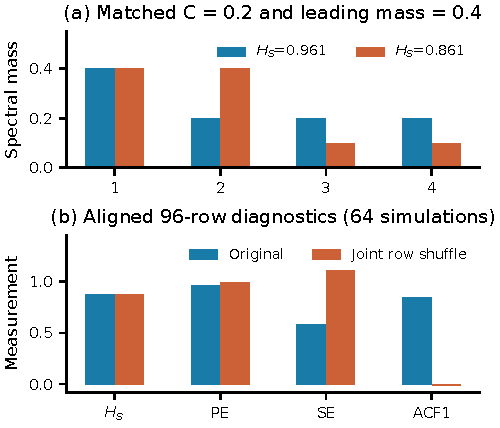
\includegraphics[width=\columnwidth]{theory.pdf}
\caption{Mathematical illustrations and aligned diagnostics, not primary fault
performance. Equal average correlation and leading concentration can coexist
with different spectral entropy. A joint time permutation preserves the
evaluated matrix while temporal measurements can change.}
\label{fig:theory}
\end{figure}

\section{Experimental Design and Audit}
The protocol and configuration were committed before full extension runs
(freeze \texttt{18b9c4a7}); original revision \texttt{b900da1b} remains
recoverable. The extension was motivated by inspected earlier findings, so
reused-data comparisons are exploratory. Exactly three primary datasets are
retained. Synthetic sizes and graph configurations are not separate datasets.

\textbf{Synthetic.} The original random geometric graphs have 64, 128 or 256
nodes. Dynamics use $x_{t+1}=(.82I-.25L/\max_i\deg_i)x_t+Bf_t+.12\epsilon_t$,
three spatially loaded OU drivers, calendar signals and burn-in 256. Spectral
radius is .82. Training data and scaling are retained, but extension development
(four 312-row simulations), calibration (32 of 256 rows) and test (four of 312
rows) use independent seeds $9000000+1000N+100s+e$. Episodes never join at
window boundaries. Synthetic display timestamps encode simulation phase.

\textbf{Intel Lab.} The original source~\cite{intel} records 54 motes at roughly
31-second cadence, with Celsius, relative humidity, lux and voltage. We retain
the original causal right-closed two-minute last-reading bins, masks and
coordinate groups. Temperature and humidity are primary; other channels remain
in the original auxiliary audit. The previously declared terminal-coverage
rule ends quantitative data before March 24, 2004; 17,970 rows retain original
60/15/10/15 chronological partitions. The four extension test blocks were
previously inspected. New injections do not make them wholly new validation.

\textbf{PEMS-BAY.} The DCRNN release~\cite{dcrnn} provides 325 road sensors,
five-minute speed in mph over January--June 2017. The retained preprocessing
expands 12 timestamp-gap rows, masks 521 zeros under release evaluation
convention and retains published road distances. Per-value upstream imputation
provenance is unavailable. The 52,128-row grid uses chronological 60/15/10/15
partitions. Extension blocks exclude original primary blocks and the original
six-unit fidelity audit. A subsequent provenance audit found that the original
long-window global diagnostic had nevertheless inspected every selected block.
Both real-data extensions therefore reuse inspected backgrounds. These are unlabelled real backgrounds
with semi-synthetic injections, not verified physical faults.

All normalizers use training medians and IQR/1.349 with documented fallbacks.
Missing neural inputs use zero plus a mask; statistical estimators retain NaN.
No observation is filled from a neighboring sensor. No window crosses a split.
Real calibration partitions were already used in the original exploratory
study; the extension's new family thresholds are fitted there without test
labels. Fitted models and groups are frozen. Calibration has 32 synthetic,
10 Intel and 31 PEMS issuances; minimum rank p-values are .0303, .0909 and .03125.
Intel therefore has a particularly coarse operating point at nominal .10.

The heterogeneous benchmark retains 12 mechanisms: copying, common interference,
decoupling, independent noise, delay, offset/gain drift, flatline, dropout,
anticorrelated copy, mixed collapse/noise, matched-average-correlation covariance
change and marginal-preserving temporal rearrangement. Each combines severity
.6/1 with duration 12/48/96, giving 72 independently specified injection draws
per configuration, sizes 6/12 and connected/partly disconnected groups. New
fault seeds are $97100+i$; seed $98100+b$ defines controls. Synthetic coupling
loss changes the state transition using the paired clean simulation seed;
real decoupling remains observational intervention. Onset is row 192; decisions
are 167,179,$\ldots$,311. The first in-event decision is 203, already 11 samples
after onset. Untouched and legitimate synchronized-transition controls accompany
each base. Fault trials therefore comprise 90\% of this constructed evaluation; its precision is not a real-deployment base-rate estimate. Forecast contexts end before every injected onset.

An alert is a connected run of consecutive flagged decisions. Hungarian
one-to-one matching credits only an alert whose onset lies inside the event,
with no trailing tolerance or point adjustment. Unmatched early, late and
control alarms are counted in controlled-benchmark precision. Native-control
exceedances are background alerts, not certified false physical diagnoses.
Event PR area uses the declared upper precision envelope over reachable recalls
because alert merging can make event recall nonmonotone. Detection delay includes
the decision grid; measured pipeline time is reported separately.

Paired percentile intervals resample whole simulations or disjoint recording
blocks, retaining their repeated injections and three model seeds. Overlapping
windows are not independent replicates. Four blocks per configuration give
limited real-data precision, and adjacent recording blocks need not be
independent. Intervals are exploratory and unadjusted for multiple comparisons;
there is no predeclared equivalence test. We report mechanism, severity,
duration, direction and support strata, rather than infer equivalence from
failure to reject a difference.

Two scoring distinctions are documented in the audit. Original finite-component
maxima could use a level when its change was unavailable; the extension requires
both endpoints of each pair. The original matrix statistic compared current
$\R$ with its reference, whereas the extension also measures $\Delta\R$.
Original results are not silently relabeled as corrected extension results.
Original removed/shuffled-graph ablations remain in v1; the temporal extension
fixes the physical/proximity graph for its feature comparisons.
An interrupted integration attempt is included in the runtime ledger. Pure
participation batching was checked against the original weighted formula.

\section{Results}
% BEGIN GENERATED: results
\subsection{Primary comparisons and incremental benefit}
Table~\ref{tab:main} reports all scheduled events; Fig.~\ref{fig:performance}
adds paired block intervals. RQ1 has a mixed answer. Synthetic diffusion S
has lower recall than SB by -0.099 [-0.174, -0.034]; its
IoU difference is -0.010 [-0.017, -0.003].
Intel diffusion S/SB recall is 0.213/0.481, but their background
exceedances are 0.218/0.372.
PEMS bootstrap S appears stronger than SB at nominal alpha
(0.528 versus 0.005 recall), with background rates
0.301 versus 0.000.
Under the descriptive test-control cap .10, corresponding recalls become
0.069 and 0.264, at attainable rates
0.026 and 0.064.
Thus a nominal-threshold ranking is not an isolated test of feature information.
The retrospective analysis does not validate a deployable threshold.

For RQ3, synthetic bootstrap T/TB recall is 0.401/0.532,
with paired difference -0.131 [-0.313, +0.054]; unconditional IoU is
0.093/0.239.
Intel bootstrap T instead exceeds TB by +0.389 [+0.264, +0.523]
recall, but their achieved background rates differ. PE and SE are not interchangeable:
Intel bootstrap PE/SE recall is 0.310/0.380,
with IoU 0.022/0.073.
Switching Intel T to diffusion yields recall 0.060 and background
exceedance 0.288. PEMS temporal contrasts have wide
block intervals. These results do not establish a universal entropy ordering.

For RQ4, synthetic bootstrap ST improves on S by
+0.123 [+0.028, +0.230] recall, but ST minus T is
+0.008 [-0.085, +0.127]. Their primary localization rules differ;
fixed-rule alternatives are retained to distinguish feature and ranking effects.
The direct incremental comparison BST minus B is
+0.003 [+0.000, +0.008] recall for synthetic bootstrap.
The other five dataset/reference combinations have zero mean recall change at
this operating point. This is not equivalence: different feature information
can be suppressed by a maximum and its recalibrated threshold.
Synthetic bootstrap BST minus B IoU is +0.008 [+0.000, +0.017].
Both use the same combined localization rule. A saved maximum-dominance audit
shows that conventional components usually determine the final scan maximum.
The retained causal GDN adaptation has synthetic/Intel/PEMS recall
0.514/0.139/0.157, with background rates
0.135/0.436/0.038.
PEMS bootstrap raw residuals reach 0.264 recall at
0.077 background exceedance. These additional
detectors retain their disclosed support and information-access differences.
For bootstrap T, conditional versus unconditional IoU is
0.231/0.093 on synthetic,
0.195/0.076 on Intel and
0.038/0.015 on PEMS.
Mean best-overlap candidate-group IoU is
0.284/0.413/0.325,
an oracle library diagnostic rather than an upper bound on every sensor ranking.
\begin{table*}[t]\centering\small
\caption{Operational extension results at nominal $\alpha=.10$. P/R: event precision/recall; AP: event-PR envelope area; IoU includes missed events as zero. These are not matched achieved background rates. PE/SE, all comparators and common-support results are retained in the artifact.}\label{tab:main}
\begin{tabular}{llrrrrrrrrrrrr}\toprule
&&\multicolumn{4}{c}{Synthetic (three sizes)}&\multicolumn{4}{c}{Intel Lab}&\multicolumn{4}{c}{PEMS-BAY}\\
Reference&Family&P&R&AP&IoU&P&R&AP&IoU&P&R&AP&IoU\\\midrule
Block & S & 0.256 & 0.285 & 0.220 & 0.024 & 0.251 & 0.208 & 0.083 & 0.017 & 0.211 & 0.528 & 0.179 & 0.035 \\
Block & T & 0.329 & 0.401 & 0.290 & 0.093 & 0.329 & 0.389 & 0.172 & 0.076 & 0.291 & 0.389 & 0.229 & 0.015 \\
Block & ST & 0.308 & 0.409 & 0.272 & 0.075 & 0.329 & 0.389 & 0.172 & 0.070 & 0.291 & 0.389 & 0.229 & 0.018 \\
Block & B & 0.484 & 0.650 & 0.452 & 0.193 & 0.000 & 0.000 & 0.139 & 0.000 & 0.224 & 0.148 & 0.207 & 0.030 \\
Block & BST & 0.486 & 0.653 & 0.456 & 0.200 & 0.000 & 0.000 & 0.139 & 0.000 & 0.224 & 0.148 & 0.207 & 0.030 \\
\midrule
Diffusion & S & 0.197 & 0.170 & 0.196 & 0.010 & 0.158 & 0.213 & 0.086 & 0.014 & 0.373 & 0.287 & 0.281 & 0.006 \\
Diffusion & T & 0.227 & 0.318 & 0.209 & 0.044 & 0.048 & 0.060 & 0.051 & 0.002 & 0.276 & 0.403 & 0.225 & 0.011 \\
Diffusion & ST & 0.197 & 0.170 & 0.196 & 0.009 & 0.048 & 0.060 & 0.051 & 0.002 & 0.376 & 0.287 & 0.300 & 0.001 \\
Diffusion & B & 0.327 & 0.392 & 0.284 & 0.102 & 0.444 & 0.056 & 0.120 & 0.015 & 0.267 & 0.111 & 0.211 & 0.022 \\
Diffusion & BST & 0.327 & 0.392 & 0.284 & 0.103 & 0.444 & 0.056 & 0.120 & 0.011 & 0.267 & 0.111 & 0.211 & 0.022 \\
\midrule
\bottomrule\end{tabular}\end{table*}

\begin{figure*}[!tb]\centering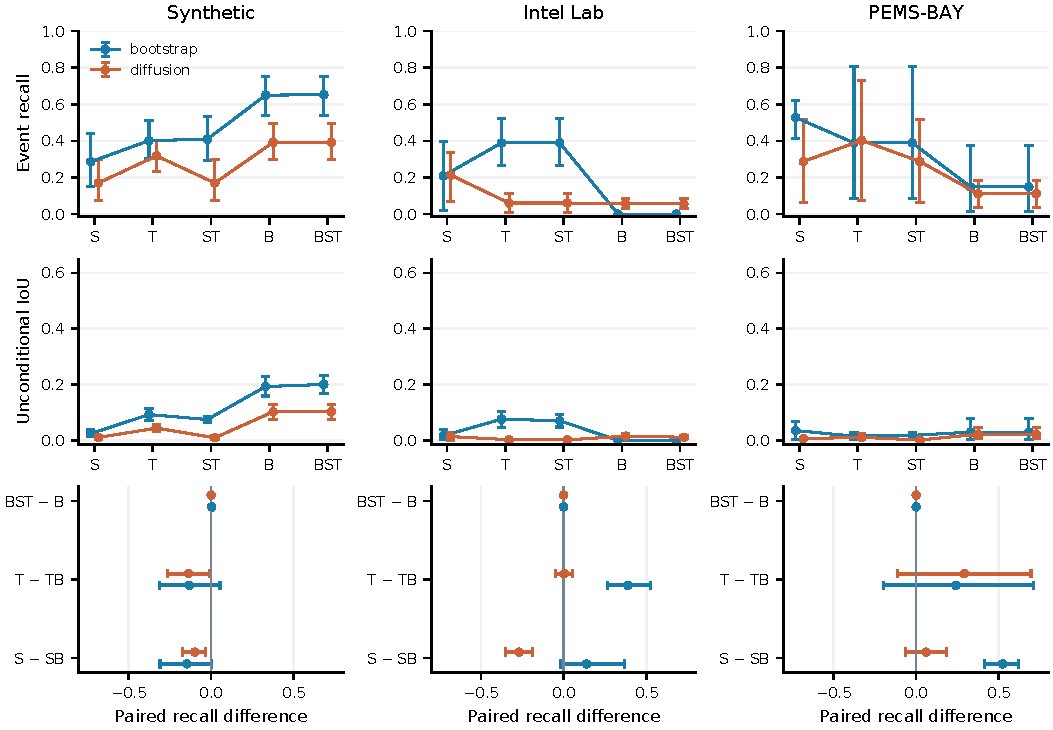
\includegraphics[width=\textwidth]{performance.pdf}
\caption{Operational performance and unadjusted paired 95\% whole-block intervals. IoU assigns zero to missed events. Equal nominal alpha does not imply equal achieved background rates; four real recording blocks give limited precision.}\label{fig:performance}\end{figure*}

\subsection{Information captured and mechanism dependence}
RQ2 is affirmative as an information distinction, not a superiority claim.
In 64 aligned simulations, joint row permutation changes the evaluated
correlation matrix by at most $1.3\times10^{-15}$ (rounded upward).
Mean PE changes from 0.964 to 0.989,
SE from 0.586 to 1.115,
and ACF1 from 0.845 to -0.016; spatial entropy is unchanged.
Conversely, copying lowers mean spatial entropy from 0.877
to 0.134, while mean PE changes only from
0.964 to 0.965.
Offsets, gains, sign changes, quantization, replay, periodic interference,
irregularity, legitimate transitions and dropout remain separate diagnostic cases.
\emph{These deliberately constructed experiments are not the primary benchmark.}

In the heterogeneous synthetic benchmark, bootstrap T/TB recall on flatlining
is 0.741/0.241;
for independent noise it is 0.463/1.000.
These are mechanism-specific operational results, not calibrated guarantees at
identical false-alert rates. A rolling window crossing a flatline onset can
remain measurable; a wholly constant window correctly abstains.
The artifact reports paired mechanism, severity, duration, measured-direction
and affected-support strata. Direction is the measured lagged change, not a
fault-name label or deviation from reference expectation. The first scheduled
in-event decision is already 11 samples late. Short events can therefore be
missed before adequate window evidence becomes available.

\begin{figure*}[!tb]\centering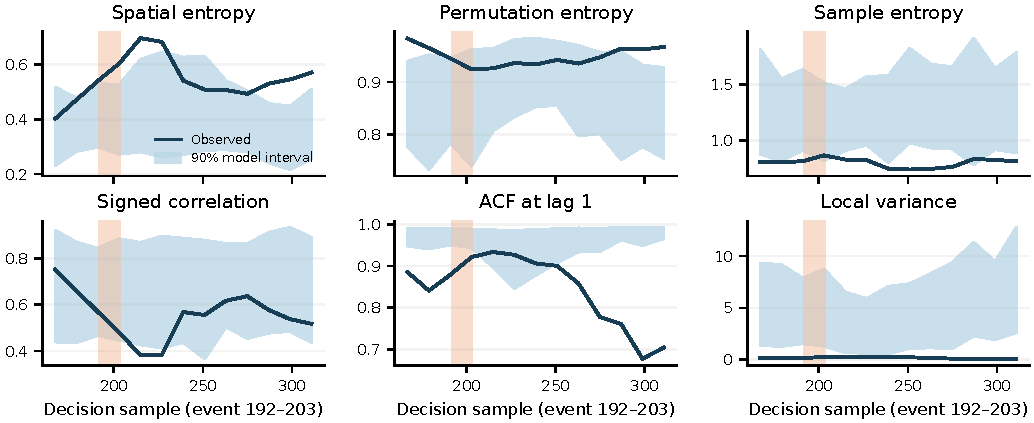
\includegraphics[width=\textwidth]{traces.pdf}
\caption{First prespecified synthetic copy episode: common forecast draws supply all bands. The first affected sensor and the best-overlap candidate group are chosen for illustration only, using injection labels; they are not a detection/localization rule. Shading marks the 12-row injection.}\label{fig:traces}\end{figure*}

\subsection{Reference fidelity, support and calibration}
For RQ5, the shared-support audit in Table~\ref{tab:fidelity} distinguishes
reference defects from feature limits. Synthetic64 diffusion spatial-entropy
coverage is 0.453
versus 0.740 for bootstrap;
Intel values are 0.083 and
1.000, on only
6.000 common spatial units per audit issuance on average.
Intel diffusion has better raw energy score
(6.336 versus 7.234),
yet its sample-entropy coverage is 0.000
versus 0.953 for bootstrap.
Good raw marginal behavior does not ensure a faithful temporal functional.
No consistent generative-reference improvement is established, and this compact
long-lead model does not represent all generative approaches.
\begin{table*}[t]\centering\small
\caption{Paired fidelity on unchanged backgrounds: seed 17, first two blocks, decisions 167/263. References share evaluated raw coordinates or eligible feature units; donor masks can still change per-draw support. Raw, H, PE, SE: 90\% coverage; TV: ordinal-pattern total variation; ES: normalized energy score (lower is better). Temporal entries use W=96. Means omit undefined units; counts and widths are saved.}\label{tab:fidelity}
\begin{tabular}{llrrrrrrrr}\toprule Dataset&Reference&Raw&H&PE&SE&ACF1 MAE&Ordinal TV&R RMSE&ES\\\midrule
Synthetic & Block & 0.875 & 0.812 & 0.855 & 0.858 & 0.034 & 0.081 & 0.236 & 0.578 \\
Synthetic & Diffusion & 0.803 & 0.513 & 0.429 & 0.222 & 0.047 & 0.150 & 0.313 & 1.747 \\
Intel Lab & Block & 0.616 & 1.000 & 0.887 & 0.953 & 0.013 & 0.378 & 0.467 & 7.234 \\
Intel Lab & Diffusion & 0.714 & 0.083 & 0.214 & 0.000 & 0.114 & 0.406 & 0.525 & 6.336 \\
PEMS-BAY & Block & 0.847 & 0.819 & 0.873 & 0.862 & 0.121 & 0.094 & 0.288 & 1.501 \\
PEMS-BAY & Diffusion & 0.739 & 0.494 & 0.699 & 0.430 & 0.163 & 0.118 & 0.360 & 2.055 \\
\bottomrule\end{tabular}\end{table*}

RQ6 exposes distinct operational and statistical limitations (Fig.~\ref{fig:availability}).
Intel S group/window eligibility is 0.017 under bootstrap
and 0.049 under diffusion; T eligibility is
0.541 and 0.633.
Per-sensor support avoids simultaneous complete rows across a group, but
availability alone does not guarantee calibrated detection. Recalibrating
on common feature support can also change achieved rates: Intel bootstrap
common-support B background exceedance is 0.551,
compared with 0.000 operationally. Varying support and nonexchangeable
calibration/test distributions remain unresolved by nominal rank calibration.

Development selects $q=3$ throughout, delay 1 for synthetic and 2 for both real
datasets; $q=4$ loses support at these short windows. Sample tolerance and group
fraction are saved per configuration. At W96, scale 2 can retain sufficient
templates, whereas scale 4 cannot meet the declared 30-template minimum;
W24 is unsupported for the primary temporal entropies. We report these as
limited multiscale support diagnostics; a separately frozen scale-2 detector
sensitivity is reported below.

\begin{figure*}[!tb]\centering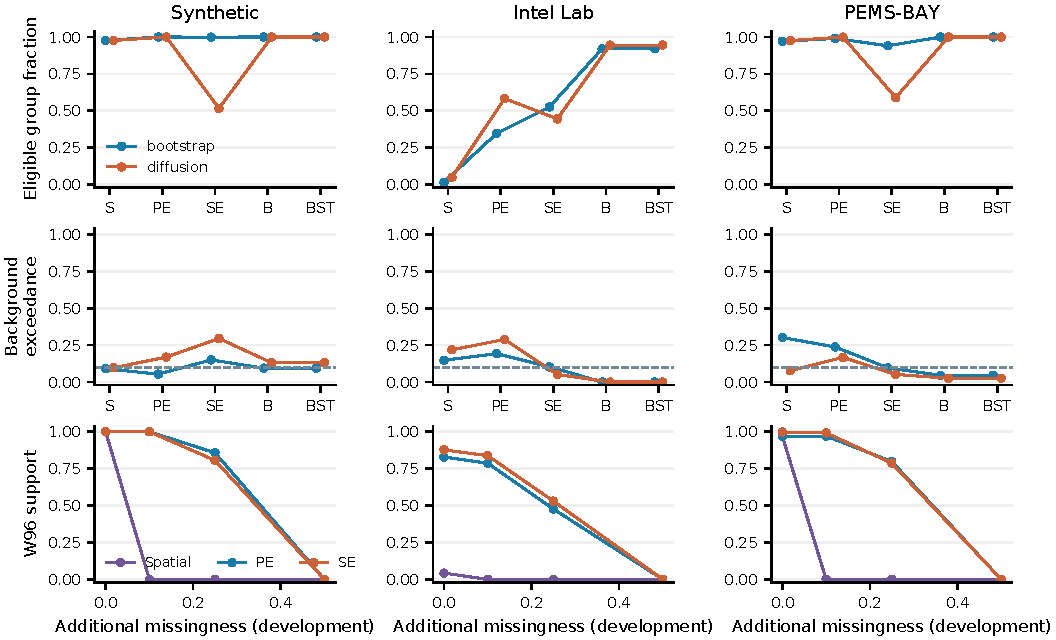
\includegraphics[width=\textwidth]{availability.pdf}
\caption{Top: operational eligible-group fraction. Middle: untouched-background exceedance at nominal alpha .10. Bottom: development-only support after independent added missingness, W96; spatial is group support, PE/SE per-sensor support. These different denominators are intentional and explicit.}\label{fig:availability}\end{figure*}

The seed-17, separately calibrated W48/W96 and 51-versus-52-reference-draw
support sensitivity completed 5 of five configurations.
Across completed configurations, the largest absolute recall change caused
by the support-rounding correction is 0.000. Window-specific thresholds
and results are retained separately; the 120-step forecast lead is held fixed.

The separately frozen, exploratory seed-17 scale-2 comparison keeps W96's
physical history, d=24 and both references. All temporal measurements use the
same two-row averages; spatial measurements remain on the original grid.
Bootstrap T recall changes (scale 2 minus 1, paired block intervals) are
-0.093 [-0.231, +0.069], -0.069 [-0.458, +0.333] and
-0.333 [-0.722, -0.028] for synthetic, Intel and PEMS. Corresponding TB
changes are -0.074 [-0.245, +0.042], +0.264 [+0.000, +0.750] and
-0.153 [-0.278, -0.028]. Full PE/SE, localization, support and achieved
background rates accompany these separately calibrated comparisons in the
artifact. Scale-1 calibration ranks reproduce the independent W96 audit;
S/SB scores are unchanged across scales. This reused-data sensitivity does
not select a new primary scale.

A post-hoc CPU estimator check uses 128 independent unit-variance
Gaussian AR(1) realizations. For independent continuous observations, PE's
between-realization SD is 0.023 at W48 and 0.009 at W96.
With fixed sample-entropy tolerance .2, finite supported fractions are
0.086 and 1.000; conditional means therefore require caution.
At $\rho=.8$, quantization to .5-unit steps yields tied-template fraction
0.653. Stable-tie PE eligibility is
0.008, versus 0.758 after discarding ties.
This demonstrates sensitivity of the quality/support decision, not a reason
to reinterpret arbitrary tied ordering as confident dynamics.
% END GENERATED: results

\section{Dashboard and Computational Artifact}
The dashboard keeps node coordinates fixed and distinguishes physical edges
from measured correlation-departure overlays. It links candidate groups to
per-sensor PE/SE, conventional temporal traces, predictive bands, actual changes,
reference departures and valid-template/pair counts. Shared channels and signed
agreement are measured descriptions. Onset-alignment summaries do not add a
decision rule. Forecast issuance, observation time, checkpoint version and
scan-calibrated p-value remain visible. Three prespecified first-copy examples
are replayed; they are not selected to maximize apparent detection success.

CUDA batches covariance, eigendecomposition, ordinal counting, conventional
statistics and joint generation. Sample-entropy pairs are chunked (512 pairs,
1024 series) to control quadratic intermediates; statistical kernels remain
float32, checked against CPU float64. Neural mixed precision is separate.
The artifact retains configuration/split/model hashes, exact prediction and
calibration arrays, per-sensor support, compact replay and all joint reference
trajectories on the experiment host. Bulky reproducible arrays are excluded
from Git; manifests and reconstruction commands describe them. Kernel timings
after warmup are distinguished from complete-pipeline latency.
% BEGIN GENERATED: compute
Isolated generation-to-score medians for synthetic64, Intel and PEMS are
0.180,
0.174 and
0.258 seconds for bootstrap, versus
0.370,
0.338 and
1.164 for diffusion on the RTX A6000.
They include generation, masks, both windows, feature extraction, scoring and
localization; they exclude GDN, acquisition, loading, disk output, rank lookup and
dashboard rendering. They are not a production end-to-end speedup claim.
Peak allocated memory in these isolated runs is at most
1.43 GiB. The PEMS temporal kernel takes
0.724 seconds on CPU float64 versus
0.035 on GPU float32, transfer excluded;
precision and hardware both differ. Maximum CPU/GPU absolute disagreement
across the benchmark is below $2.0\times10^{-7}$.
The cumulative GPU-stage ledger, including the original study, validation and
failed attempts, records 4.271 hours within the explicitly
authorized eight-hour ceiling. All primary, window/support, scale-2 and
fidelity/timing comparisons completed. The earlier four-hour stop is preserved;
CPU reporting and rendering are outside this experiment-stage ledger.

\begin{figure*}[!tb]\centering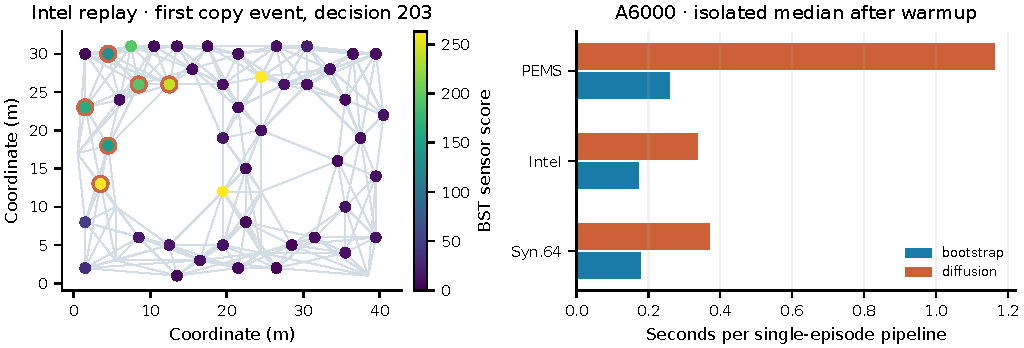
\includegraphics[width=\textwidth]{dashboard_cost.pdf}
\caption{Intel replay localization display (orange outlines: injected sensors, for evaluation only) and isolated generation-to-score timing. The example is the first prespecified copy trial, not a selected success. Timing excludes loading, acquisition and presentation.}\label{fig:dashboard-cost}\end{figure*}
% END GENERATED: compute

\section{Limitations and Conclusion}
% BEGIN GENERATED: conclusion
The comparison establishes different measurement information, but no consistent
overall entropy advantage. Temporal entropy can respond when aligned covariance
is invariant; conventional temporal statistics can respond too. Missing-data
support and reference mismatch materially affect operational results. The
Intel bootstrap temporal-entropy advantage occurs under one frozen calibration
setting with different achieved background rates, while synthetic conventional
temporal localization is stronger. Augmenting conventional features changes
synthetic bootstrap recall by 0.003 and leaves recall unchanged in the
other primary dataset/reference combinations. This limited incremental effect
under a maximum rule does not establish statistical or practical equivalence.
The evaluated diffusion reference shows no consistent improvement over joint
bootstrap; its feature-distribution failures cannot establish that entropy
itself is intrinsically inadequate.
% END GENERATED: conclusion
The real-data study is semi-synthetic and partly reuses inspected recordings;
it cannot establish sensitivity to verified native faults. Compact diffusion
forecasts at long lead, model-specific support, limited calibration units,
four real recording blocks and a finite neighborhood library constrain the
comparison. Unsupported sample entropy is retained as a limitation, not silently
replaced. Longer multiscale histories would need equally long conventional
comparators and new forecasting/calibration evaluation. Native causes and
dashboard usability are not validated by injected labels.

\section*{Acknowledgment and AI disclosure}
OpenAI Codex assisted implementation, experiment orchestration, analysis code,
figure generation and drafting throughout this work. Numerical results come
from the saved experiments and stated proofs; the authors retain responsibility
for verification and final submission. The diffusion reference is a separate
scientific model described in the methods. We acknowledge the original Intel
Lab data collectors and the DCRNN release authors.
% Balance the final two columns with the standard IEEEtran bibliography hook.
\IEEEtriggeratref{7}
\bibliographystyle{IEEEtran}
\bibliography{references}
\end{document}
